Una parte necesaria para entender la capa física del modelo OSI es el de los tipos de medios de transmisión de datos, en este caso haré un vistazo a los \textit{Medios de Transmisión Guiados.} 
Para comenzar hay que recordar que el medio en un sistema de transmisión de datos, es la ruta física entre el transmisor y el receptor. Con esta definición podemos decir que un \textbf{medio de transmisión guiado} es llamado así debido a que la señal que viaja a través de cualquiera de estos medios está dirigida y contenida por los límites físicos del medio.
\section{Tipos de Medios de Transmisión Guiados}
En general hay 3 tipos de medios guiados (Data Communications And Networking 4th Edition, Behrouz A. Forouzan): \\
\begin{center}
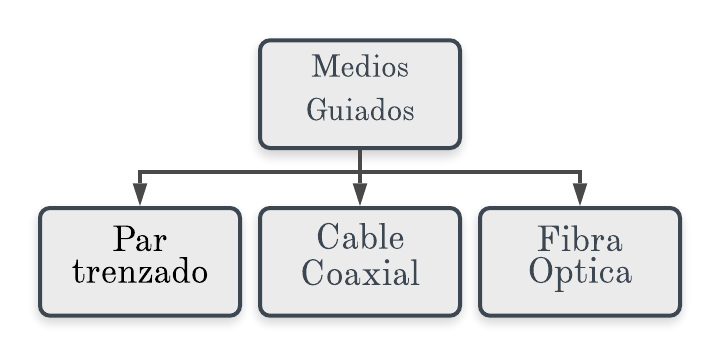
\includegraphics[scale=0.25]{D1}
\end{center}
\subsection{Par Trenzado}
Este es el medio de transmisión menos costoso y mas utilizado.
\subsubsection{Descripción Física}
Un par trenzado consta de dos alambres de cobre aislados, típicamente de aproximadamente 1 mm de espesor. Los cables están retorcidos en forma helicoidal, como una molécula de ADN Por lo general, varios de estos pares se agrupan en un cable envolviéndolos en una cubierta protectora resistente. En distancias más largas, los cables pueden contener cientos de pares.
\begin{figure}[!ht]
\centering
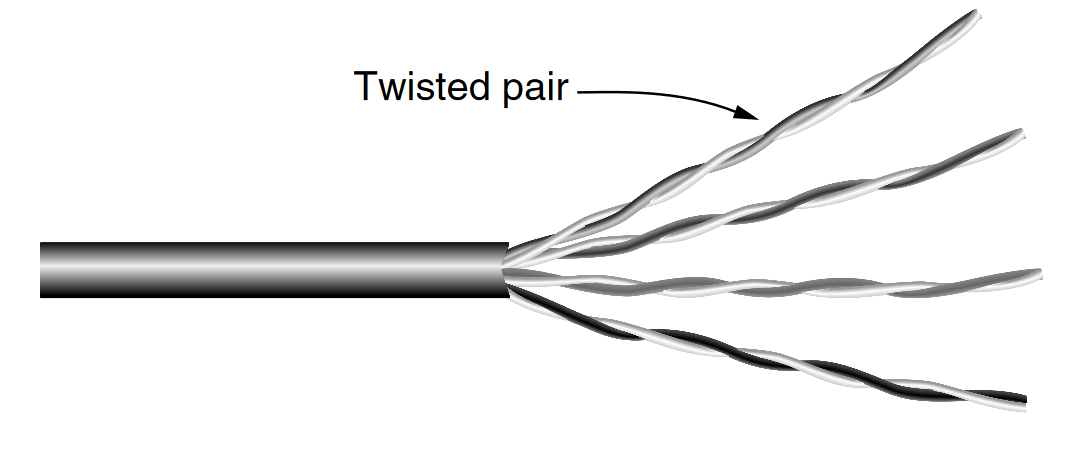
\includegraphics[scale=0.5]{D2}
\caption{Cable \texttt{UTP} con cuatro pares trenzados.}
\end{figure}
\subsubsection{Aplicaciones}
Es el medio de transmisión más común para señales analógicas y digitales ademas es utilizado en la red telefónica y es el caballo de batalla para las comunicaciones dentro de los edificios.
\subsubsection{Ventajas y Desventajas}

\begin{center}
\begin{tabular}{*2l}
\toprule
Ventajas &   {} \\
\midrule
\texttt{UTP} & {} \\
Instalación & Facil de Curvar\\

Costo & Accesible\\

Conector & Confiable\\
\texttt{STP} & {} \\
Interferencia & Baja susceptibilidad \\
Conector & Poco Confiable \\
{}&{}\\
\bottomrule
\end{tabular}
\quad
\begin{tabular}{*2l}
\toprule
Desventajas &   {} \\
\midrule
{} & {} \\
Distancias   & $\approx$100m   \\
Interferencias   &  Alta Susceptibilidad\\
Instalación   &  Curvas Complicadas\\
{} & {} \\
Distancia & $\approx$100m\\
Instalación & Dificil de Curvar\\
Costo & Moderadamente alto\\
\bottomrule
\end{tabular}
\end{center}
\subsection{Cable Coaxial}
\subsubsection{Descripción Física}
El cable coaxial, como el par trenzado, consta de dos conductores, pero está construido de manera diferente para permitirle operar en un rango más amplio de frecuencias. Consiste en un conductor cilíndrico exterior que se encuentra debajo de un único conductor de cable interno.
\begin{figure}[!ht]
\centering
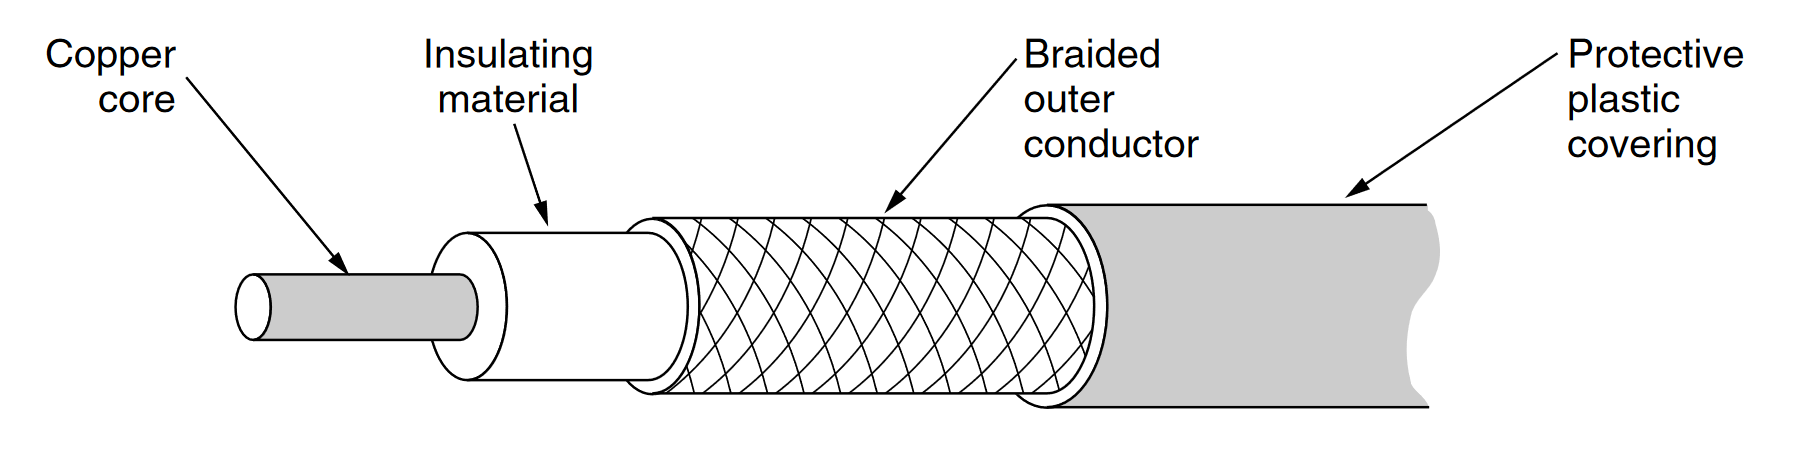
\includegraphics[scale=0.45]{D3}
\caption{Cable Coaxial}
\end{figure}
\subsubsection{Aplicaciones}
El cable coaxial es quizás el medio de transmisión más versátil y goza de un uso generalizado en una amplia variedad de aplicaciones. Los más importantes de estos son:
\begin{itemize}
\item Distribución televisiva
\item Transmisión telefónica de larga distancia
\item Enlaces de sistema informático de corto plazo
\item Redes de área local
\end{itemize}
\subsubsection{Ventajas y Desventajas}
\begin{center}
\begin{tabular}{*2l}
\toprule
Ventajas &   {} \\
\midrule
Distancia   & $\approx$180m   \\
Costo   &  Muy Barato \\
Interferencia   &  Poco Susceptible \\
\bottomrule
\end{tabular}
\quad
\begin{tabular}{*2l}
\toprule
Desventajas &   {} \\
\midrule
Instalación   & Difícil de Curvar   \\
Conector   &  Poco confiable \\
Perdidas   &  Altas en conectores \\
\bottomrule
\end{tabular}
\end{center}
\subsection{Fibra Óptica}
\subsubsection{Descripción Física}
Una fibra óptica es un medio delgado (de 2 a 125$\mu$m), flexible, capaz de guiar un rayo óptico. Se pueden usar varios vidrios y plásticos para hacer fibras ópticas. Un cable de fibra óptica tiene una forma cilíndrica y consta de tres secciones concéntricas: el núcleo, el revestimiento y la cubierta. El núcleo es la sección más interna y consta de uno o más hilos muy delgados, o fibras, hechas de vidrio o plástico; el núcleo tiene un diámetro en el rango de 8 a 100 $\mu$m. Cada fibra está rodeada por su propio revestimiento, un recubrimiento de vidrio o plástico que tiene propiedades ópticas diferentes de las del núcleo. La interfaz entre el núcleo y el revestimiento actúa como un reflector para confinar la luz que de otro modo escaparía del núcleo. La capa más externa, que rodea una o un conjunto de fibras revestidas, es la chaqueta. La chaqueta está compuesta de plástico y otros materiales en capas para proteger contra la humedad, la abrasión, el aplastamiento y otros peligros ambientales.
\begin{figure}[!ht]
\centering
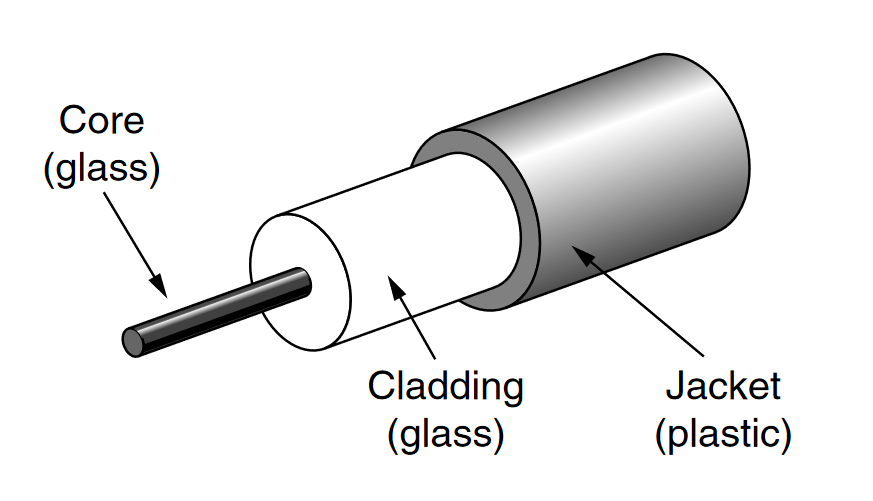
\includegraphics[scale=0.45]{D4}
\caption{Una sola fibra.}
\end{figure}
\subsubsection{Aplicaciones}
Aquí tenemos algunas aplicaciones de la fibra óptica:
\begin{itemize}
\item \textbf{Médico}: Utilizado como guías de luz, herramientas de imagen y también como láser para cirugías.
\item \textbf{Defensa / Gobierno:} Utilizado para ondas sísmicas y SONAR, como cableado en aviones, submarinos y otros vehículos y también para redes de campo.
\item \textbf{Proveedores de Servicios:} Las compañías de transmisión / cable están utilizando cables de fibra óptica para el cableado HDTV, internet, vídeo a pedido y otras aplicaciones.
\item \textbf{Industrial / Comercial:} Se utiliza para obtener imágenes en áreas de difícil acceso, como dispositivos sensoriales para realizar mediciones de temperatura, presión y otras, y como cableado en automóviles y en entornos industriales.
\end{itemize}
\subsubsection{Forma de Transmisión de Datos}
La fibra óptica de una manera simplificada funciona transmitiendo un haz de luz codificado por señal por medio de una reflexión interna total, es decir, se ''lanza'' un rayo dentro del cable y este rebota en las paredes internas del mismo hasta llegar al receptor. Y hay tres maneras en que este proceso es realizado:
\begin{itemize}
\item \textbf{Modo Simple:}
\begin{figure}[!ht]
\centering
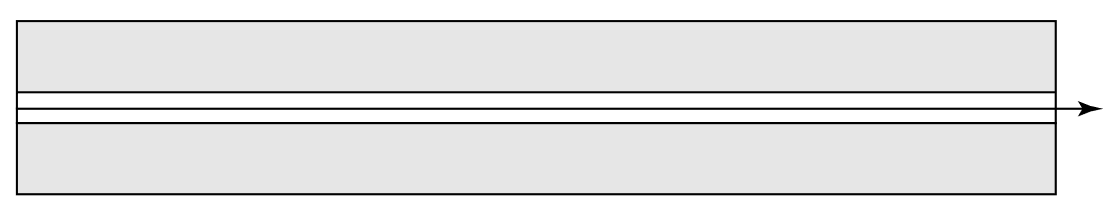
\includegraphics[scale=0.45]{D5}
\caption{Simple}
\end{figure}
\item \textbf{Multimodo:}
\begin{figure}[!ht]
\centering
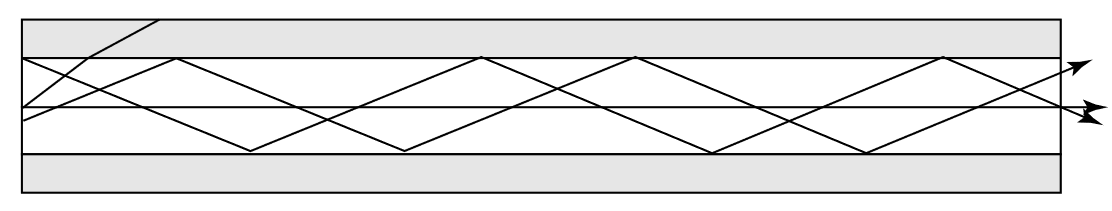
\includegraphics[scale=0.45]{D6}
\caption{Multimodo}
\end{figure}
\item \textbf{Multimodo Indice Gradual:}
\begin{figure}[!ht]
\centering
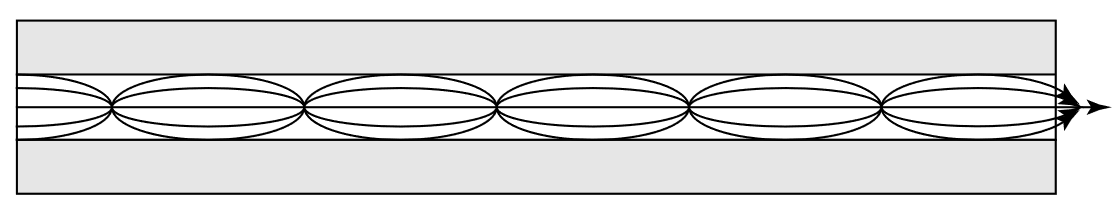
\includegraphics[scale=0.45]{D7}
\caption{Multimodo Indice Gradual}
\end{figure}
\end{itemize}
\subsubsection{Ventajas y Desventajas}

\begin{center}
\begin{tabular}{*2l}
\toprule
Ventajas &   {} \\
\midrule
Distancia   & $\approx$2Km - 100Km   \\
Conector   &  Confiable \\
Interferencia   &  Nula \\
\bottomrule
\end{tabular}
\quad
\begin{tabular}{*2l}
\toprule
Desventajas &   {} \\
\midrule
Costo   & Elevado   \\
Instalación   &  Empalmes\\
Instalación   &  Curvas Complicadas\\
\bottomrule
\end{tabular}
\end{center}